\section{Functional View}

\begin{figure}[H]
    \centering
    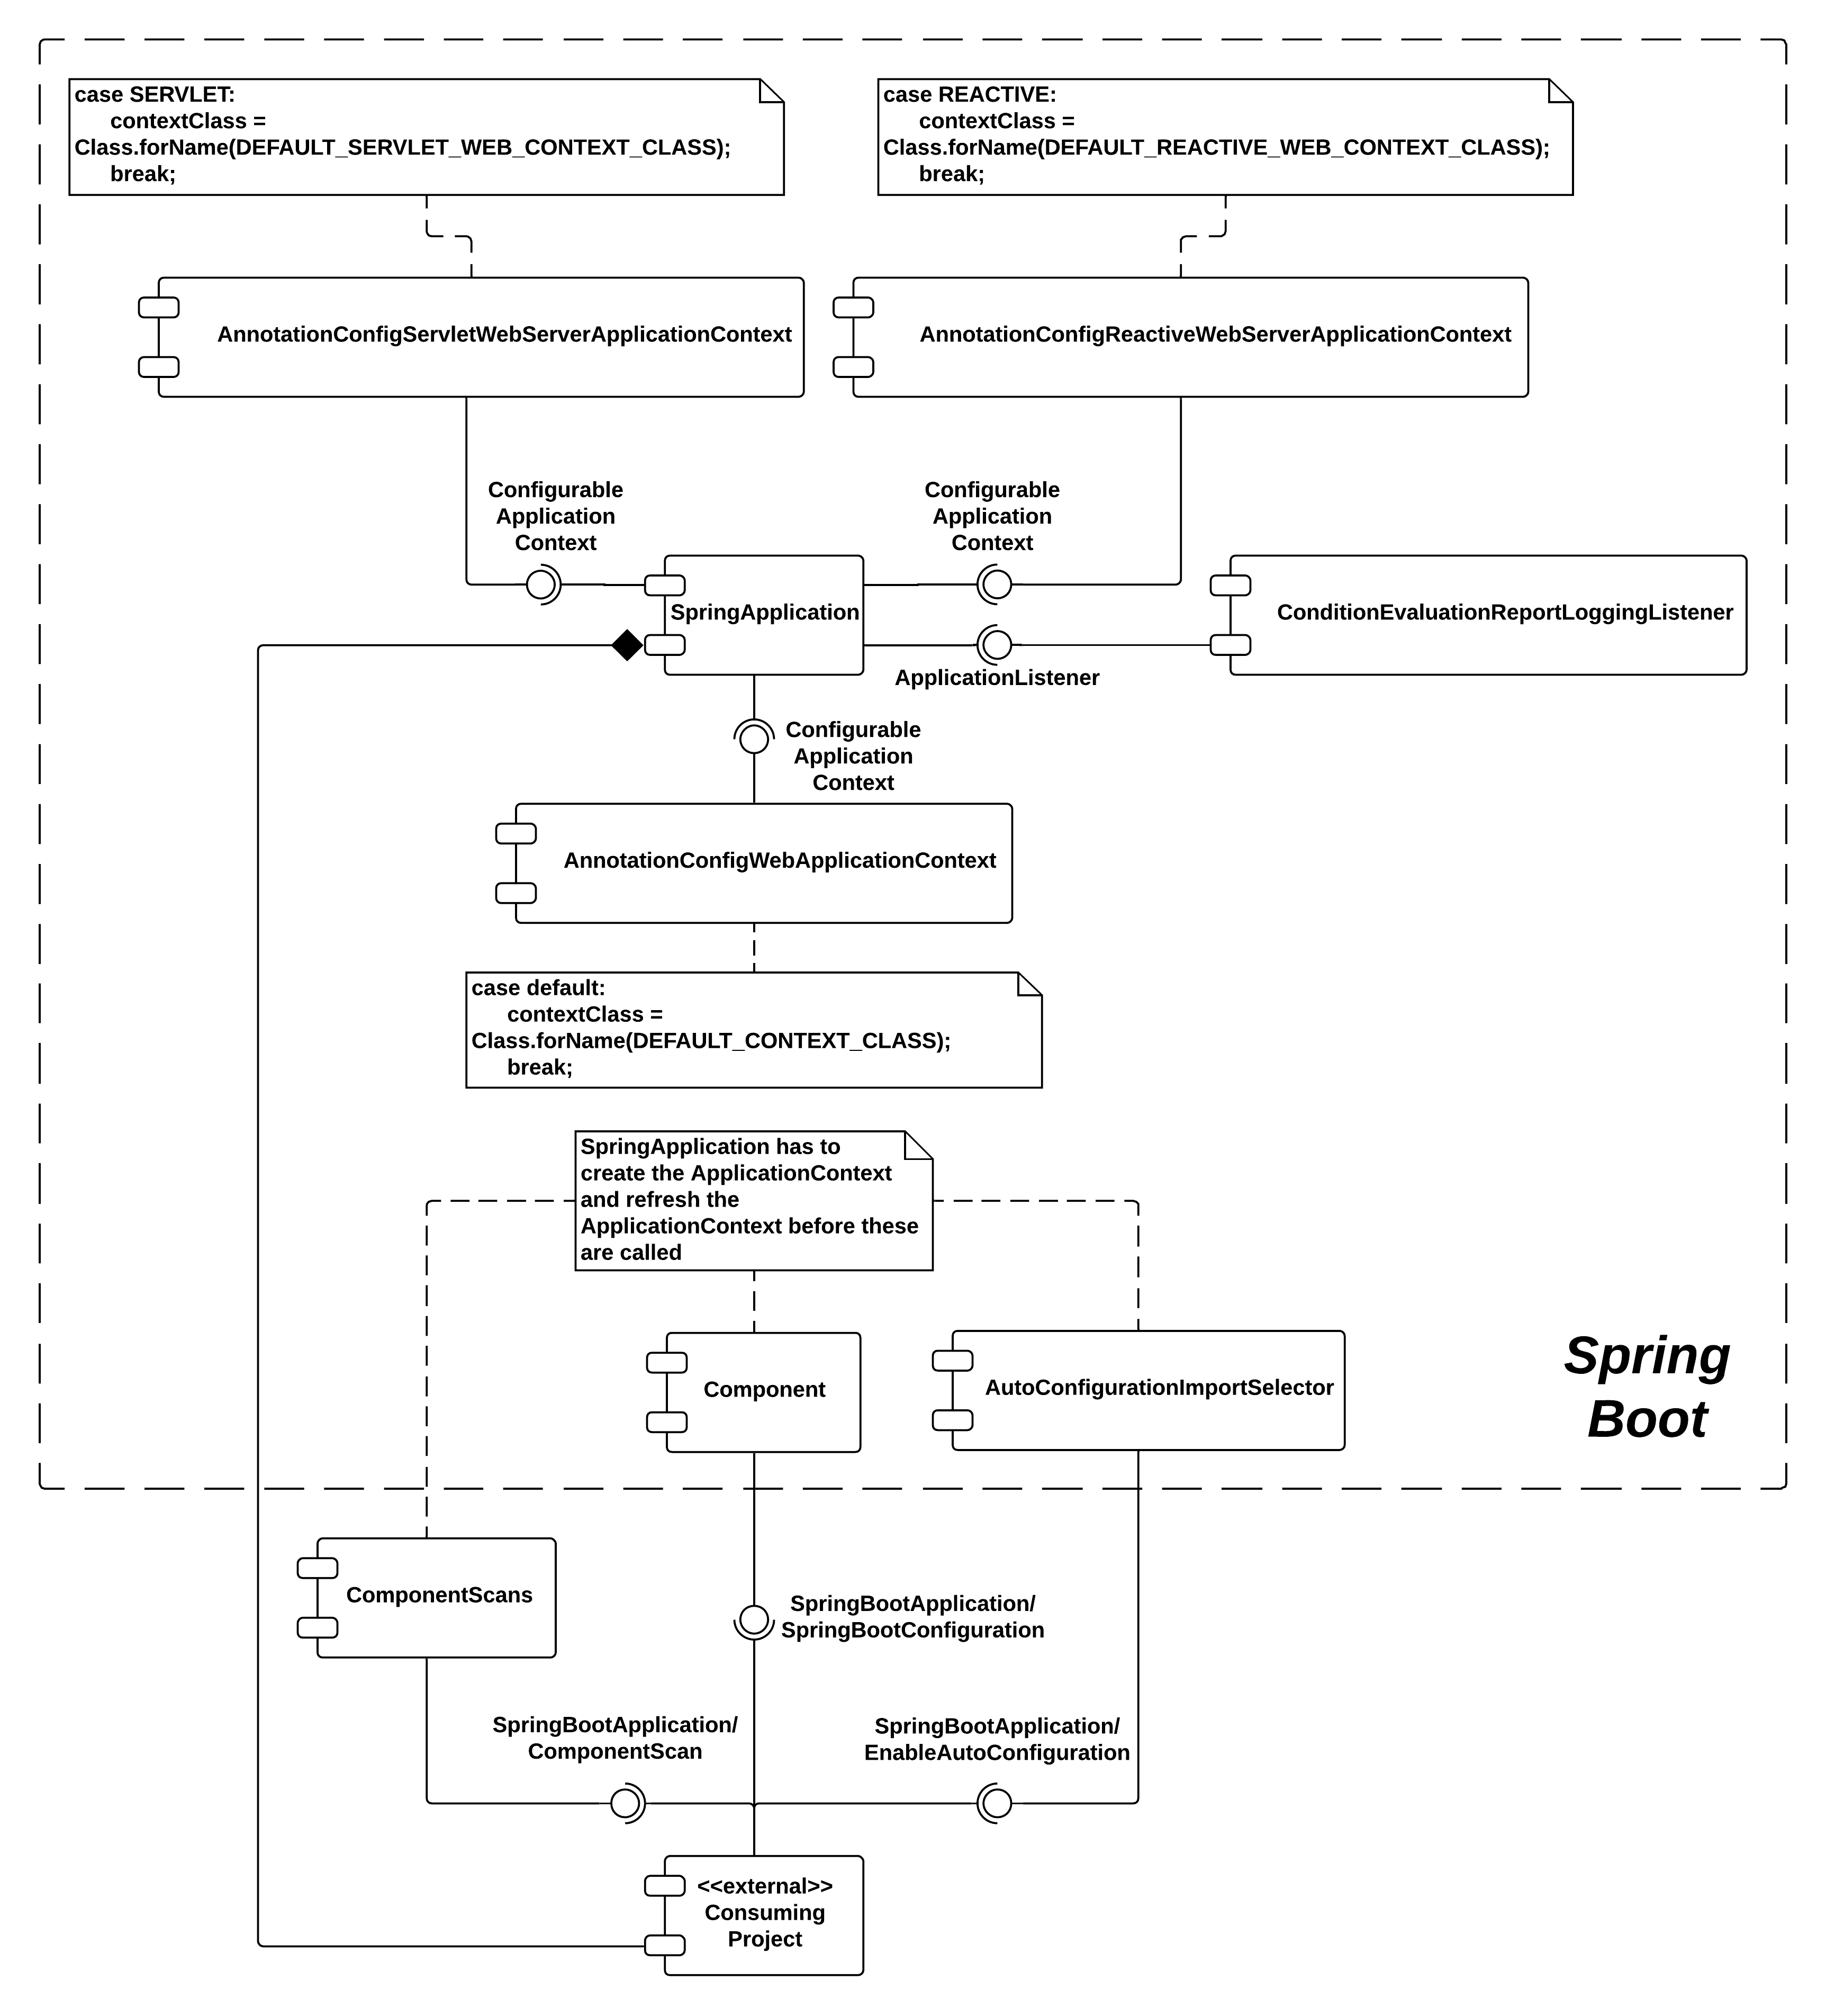
\includegraphics[width=.9\textwidth]{content/architectural-views-top-level/spring-boot-component-diagram.png}
    \caption{Spring Boot Component Diagram}
    \label{component-diagram}
\end{figure}

Spring Boot leverages some functionalities of Spring Framework and takes an opinionated stance of building Spring web applications. It is important to point out the opinion of Spring Boot, because this is the primary reason that it removes the burden of developing boilerplate configurations.  It does so with the \texttt{@SpringBootApplication} annotation that extends the interfaces -- EnableAutoConfiguration, SpringBootConfiguration and ComponentScan -- to give the user an easier experience for setting up a web application. They do not have to completely understand the magic that happens behind the scene but reap the benefit of the abstraction.

Spring Boot enacts the following tasks in sequence when a consuming project initiates a start-up using \texttt{SpringApplication.run()}:

\begin{enumerate}
\item The application context starts.
\item A component scan occurs with the \texttt{@ComponentScan} annotation -- which is a functionality of Spring Framework -- and discovers all subpackages relative to the consuming project's application class.
\item The \texttt{@SpringBootConfiguration} annotation will use the discovered subpackages as its' scope for instantiating and configuring pre-defined beans within it.
\item The \texttt{@EnableAutoConfiguration} annotation instantiate beans based on the dependencies in the classpath. It will also match the dependencies in the classpath and compare it to the \texttt{spring.factories} properties, which then evaluates conditionals based on a match to check whether auto-configuration is necessary.
\end{enumerate}

\subsection{Functional Elements}

As a reference point for Listings~\ref{AnnotationConfigServletWebServerApplicationContext},~\ref{AnnotationConfigReactiveWebServerApplicationContext}, and~\ref{AnnotationConfigApplicationContext}, Listing~\ref{ApplicationContext} shows Spring Boot's code that contains a Java switch case statement which determines the application context based on the web application type of the consuming project. To give a little more context, the web application type is deduced from the classpath dependencies. On a high level, each of the application context are resolved to with the following in their classpath:

\begin{itemize}
\item \texttt{javax.servlet.Servlet} or\\\texttt{org.springframework.web.context.ConfigurableWebApplicationContext} resolves to a \texttt{SERVLET} application context.
\item \texttt{org.springframework.web.servlet.DispatcherServlet} resolves to a \texttt{REACTIVE} application context.
\item If none of the above are present in the classpath, Spring Boot will resolve to a default application context.
\end{itemize}

\clearpage

\begin{lstlisting}[language=Java, caption={Determination of Application Context \cite{createapplicationcontext:online}}, label=ApplicationContext]

protected ConfigurableApplicationContext createApplicationContext() {
	Class<?> contextClass = this.applicationContextClass;
	if (contextClass == null) {
		try {
			switch (this.webApplicationType) {
			case SERVLET:
				contextClass = Class.forName(DEFAULT_SERVLET_WEB_CONTEXT_CLASS);
				break;
			case REACTIVE:
				contextClass = Class.forName(DEFAULT_REACTIVE_WEB_CONTEXT_CLASS);
				break;
			default:
				contextClass = Class.forName(DEFAULT_CONTEXT_CLASS);
			}
		}
		catch (ClassNotFoundException ex) {
			throw new IllegalStateException(
					"Unable create a default ApplicationContext, please specify an ApplicationContextClass", ex);
		}
	}
	return (ConfigurableApplicationContext) BeanUtils.instantiateClass(contextClass);
}
	
\end{lstlisting}\ \\

The following are the list of most common functional elements of Spring Boot:
{
\obeylines
\setlength\parindent{0pt}

\noindent\makebox[\linewidth]{\rule{\textwidth}{3pt}}\ \\

\textbf{Element Name}: AutoConfigurationImportSelector\\
\textbf{Description}: AutoConfigurationImportSelector uses an interface called EnableAutoConfiguration. The EnableAutoConfiguration interface is extended by the SpringBootApplication interface, which uses the auto-configuration classes inside of the \texttt{spring.factories} properties and are applied based on dependencies in the classpath. This mechanism for applying the auto-coonfigurations is done through the \texttt{SpringFactoriesLoader} class under the \texttt{org.springframework.core.io.support} package which iterates over \texttt{spring.factories} file properties living inside of the \texttt{org.springframework.boot.autoconfigure} package. The iteration process is looking for matches to the Auto-configuration classes, then evaluates the conditionals in each of those matching classes such as \texttt{@ConditionalOnClass}. EnableAutoConfiguration also has ways in which users can exclude any configuration that do not need to be applied. There are two ways to exclude auto-configuration of specific dependencies by using the \texttt{exclude()} and \texttt{excludeName()} methods within EnableAutoConfiguration.\\
\textbf{Interface}: The consumer project's application class with the \texttt{main} method that invokes \texttt{SpringApplication.run()}:\\

\begin{lstlisting}[language=Java, caption=Consumer Project Auto-Configuring Dependencies using SpringBootApplication]

import org.springframework.boot.autoconfigure.mongo.MongoAutoConfiguration;
import org.springframework.boot.autoconfigure.data.mongo.MongoDataAutoConfiguration;
import org.springframework.boot.SpringApplication;
import org.springframework.boot.autoconfigure.SpringBootApplication;

@SpringBootApplication(exclude =
	MongoAutoConfiguration.class,
    MongoDataAutoConfiguration.class
)
public class ConsumerProjectApplication {
	public static void main(String[] args) {
        SpringApplication.run(ConsumerProjectApplication.class, args);
    }
}
\end{lstlisting}\ \\

The code above uses the \texttt{@SpringBootApplication} annotation and passes in the list of classes to exclude. The reason \texttt{@SpringBootApplication} is able to do this is because internally it aliases EnableAutoConfiguration which contains the \texttt{exclude()} and \texttt{excludeName()} methods. In this case, it is excluding \texttt{MongoAutoConfiguration.class} and \texttt{MongoDataAutoConfiguration.class}. By default, it will auto-configure the dependencies in the classpath.\\

An alternate way of achieving the same outcome would be the following code below:\\

\begin{lstlisting}[language=Java, caption=Consumer Project Auto-Configuring Dependencies using EnableAutoConfiguration, label=AutoConfigurationImportSelector]

import org.springframework.boot.autoconfigure.mongo.MongoAutoConfiguration;
import org.springframework.boot.autoconfigure.data.mongo.MongoDataAutoConfiguration;
import org.springframework.boot.autoconfigure.EnableAutoConfiguration;
import org.springframework.boot.SpringApplication;

@EnableAutoConfiguration(exclude =
	MongoAutoConfiguration.class,
    MongoDataAutoConfiguration.class
)
public class ConsumerProjectApplication {
	public static void main(String[] args) {
        SpringApplication.run(ConsumerProjectApplication.class, args);
    }
}
\end{lstlisting}\ \\

\noindent\makebox[\linewidth]{\rule{\textwidth}{3pt}}\ \\

\textbf{Element Name}: AnnotationConfigServletWebServerApplicationContext\\
\textbf{Description}: The consumer project's application class with the \texttt{main} method that invokes \texttt{SpringApplication.run()} uses the \texttt{createApplicationContext} method that abides by the strategy pattern to determine the application context to create based on the web application type. In the case that the web application type is found to be \texttt{SERVLET} by means of the \texttt{deduceFromClasspath} method, then the \texttt{AnnotationConfigServletWebServerApplicationContext} class will create the application context. Essentially as described by the Spring javadoc, "the application that should run as a servlet-based web application" \cite{springjavadoc:onlineWebApplicationType}.\\
\textbf{Interface}: The consumer project's application class with the \texttt{main} method that invokes \texttt{SpringApplication.run()}:\\

\begin{lstlisting}[language=Java, caption=Creating application context for servlet-based web application, label=AnnotationConfigServletWebServerApplicationContext]

import org.springframework.boot.SpringApplication;
import org.springframework.boot.autoconfigure.SpringBootApplication;

@SpringBootApplication
public class ConsumerProjectApplication {
    public static void main(String[] args) {
        SpringApplication.run(ConsumerProjectApplication.class, args);
    }
}
\end{lstlisting}\ \\

\texttt{SpringApplication.run()} method creates application context using the interface \texttt{ConfigurableApplicationContext} which is implemented by  \texttt{ServletWebServerApplicationContext} class. The \texttt{ServletWebServerApplicationContext} class is extended by \texttt{AnnotationConfigServletWebServerApplicationContext} to help in creating the servlet web server application context.\\

\noindent\makebox[\linewidth]{\rule{\textwidth}{3pt}}\ \\

\textbf{Element Name}: AnnotationConfigReactiveWebServerApplicationContext\\
\textbf{Description}: The consumer project's application class with the \texttt{main} method that invokes \texttt{SpringApplication.run()} uses the \texttt{createApplicationContext} method that abides by the strategy pattern to determine the application context to create based on the web application type.
In the case that the web application type is found to be \texttt{REACTIVE} by means of the \texttt{deduceFromClasspath} method, then the \texttt{AnnotationConfigReactiveWebServerApplicationContext} class will create the application context. Essentially as described by the Spring javadoc, "the application that should run as a reactive web application" \cite{springjavadoc:onlineAnnotationConfigReactiveWebServerApplicationContext}.\\
\textbf{Interface}: The consumer project's application class with the \texttt{main} method that invokes \texttt{SpringApplication.run()}:\\

\clearpage

\begin{lstlisting}[language=Java, caption=Creating application context for reactive web application, label=AnnotationConfigReactiveWebServerApplicationContext]

import org.springframework.boot.SpringApplication;
import org.springframework.boot.autoconfigure.SpringBootApplication;

@SpringBootApplication
public class ConsumerProjectApplication {
    public static void main(String[] args) {
        SpringApplication.run(ConsumerProjectApplication.class, args);
    }
}
\end{lstlisting}\ \\

\texttt{SpringApplication.run()} method creates application context using the interface \texttt{ConfigurableApplicationContext} which is implemented by  \texttt{ReactiveWebServerApplicationContext} class. The \texttt{ReactiveWebServerApplicationContext} class is extended by \texttt{AnnotationConfigReactiveWebServerApplicationContext} to help in creating the application context for the reactive web application.\\

\noindent\makebox[\linewidth]{\rule{\textwidth}{3pt}}\ \\

\textbf{Element Name}: AnnotationConfigApplicationContext\\
\textbf{Description}: The consumer project's application class with the \texttt{main} method that invokes \texttt{SpringApplication.run()} uses the \texttt{createApplicationContext} method that abides by the strategy pattern to determine the application context to create based on the web application type. In the case that the web application type is not found to be \texttt{REACTIVE} or \texttt{SERVLET} by means of the \texttt{deduceFromClasspath} method, then the \texttt{AnnotationConfigApplicationContext} class will create the application context. Essentially as described by the Spring javadoc, "The application should not run as a web application" \cite{springjavadoc:onlineAnnotationConfigApplicationContext}.\\
\textbf{Interface}: The consumer project's application class with the \texttt{main} method that invokes \texttt{SpringApplication.run()}:\\

\clearpage

\begin{lstlisting}[language=Java, caption=Creating application context for non-web application, label=AnnotationConfigApplicationContext]

import org.springframework.boot.SpringApplication;
import org.springframework.boot.autoconfigure.SpringBootApplication;

@SpringBootApplication
public class ConsumerProjectApplication {
    public static void main(String[] args) {
        SpringApplication.run(ConsumerProjectApplication.class, args);
    }
}
\end{lstlisting}\ \\

\texttt{SpringApplication.run()} method creates application context using the \texttt{AnnotationConfigApplicationContext} class which implements the \texttt{ConfigurableApplicationContext} interface.\\

\noindent\makebox[\linewidth]{\rule{\textwidth}{3pt}}\ \\

\textbf{Element Name}: Component\\
\textbf{Description}: The \texttt{Component} class implements the \texttt{SpringBootConfiguration} interface. The \texttt{SpringBootConfiguration} interface is extended by the \texttt{SpringBootApplication} interface which is used for configuring the consumer project's pre-defined beans. The \texttt{SpringBootConfiguration} interface also has an explicit way to specify the name of the Spring bean by.\\
\textbf{Interface}: The consumer project's application class with the \texttt{main} method that invokes \texttt{SpringApplication.run()}:\\

\clearpage

\begin{lstlisting}[language=Java, caption=Consumer Project creating pre-defined beans using SpringBootApplication]

import org.springframework.boot.SpringApplication;
import org.springframework.boot.autoconfigure.SpringBootApplication;
import org.springframework.context.annotation.Bean;
import org.springframework.web.client.RestTemplate;

@SpringBootApplication
public class ConsumerProjectApplication {
    public static void main(String[] args) {
        SpringApplication.run(ConsumerProjectApplication.class, args);
    }
    
    @Bean
    public RestTemplate restTemplate() {
        return new RestTemplate();
    }
}
\end{lstlisting}\ \\

\clearpage

An alternate way of achieving the same outcome would be the following code below:\\

\begin{lstlisting}[language=Java, caption=Consumer Project creating pre-defined beans using SpringBootConfiguration]

import org.springframework.boot.SpringApplication;
import org.springframework.boot.autoconfigure.SpringBootConfiguration;
import org.springframework.context.annotation.Bean;
import org.springframework.web.client.RestTemplate;

@SpringBootConfiguration
public class ConsumerProjectApplication {
    public static void main(String[] args) {
        SpringApplication.run(ConsumerProjectApplication.class, args);
    }
    
    @Bean
    public RestTemplate restTemplate() {
        return new RestTemplate();
    }
}
\end{lstlisting}\ \\

\noindent\makebox[\linewidth]{\rule{\textwidth}{3pt}}
}\ \\

These functional elements depict the internal workings of Spring Boot to achieve quick and easy configuration experience for users and their consuming project. The abstractions are meant to assist users and not confuse them, which is why they are not readily exposed to them. All if not most software frameworks will do this to ease the experience of software development. To properly show how Spring Boot functional elements interact with each other, it is important to show the sequence of operations with diagrams.

\subsection{Sequence Diagrams}
\begin{figure}[H]
    \centering
    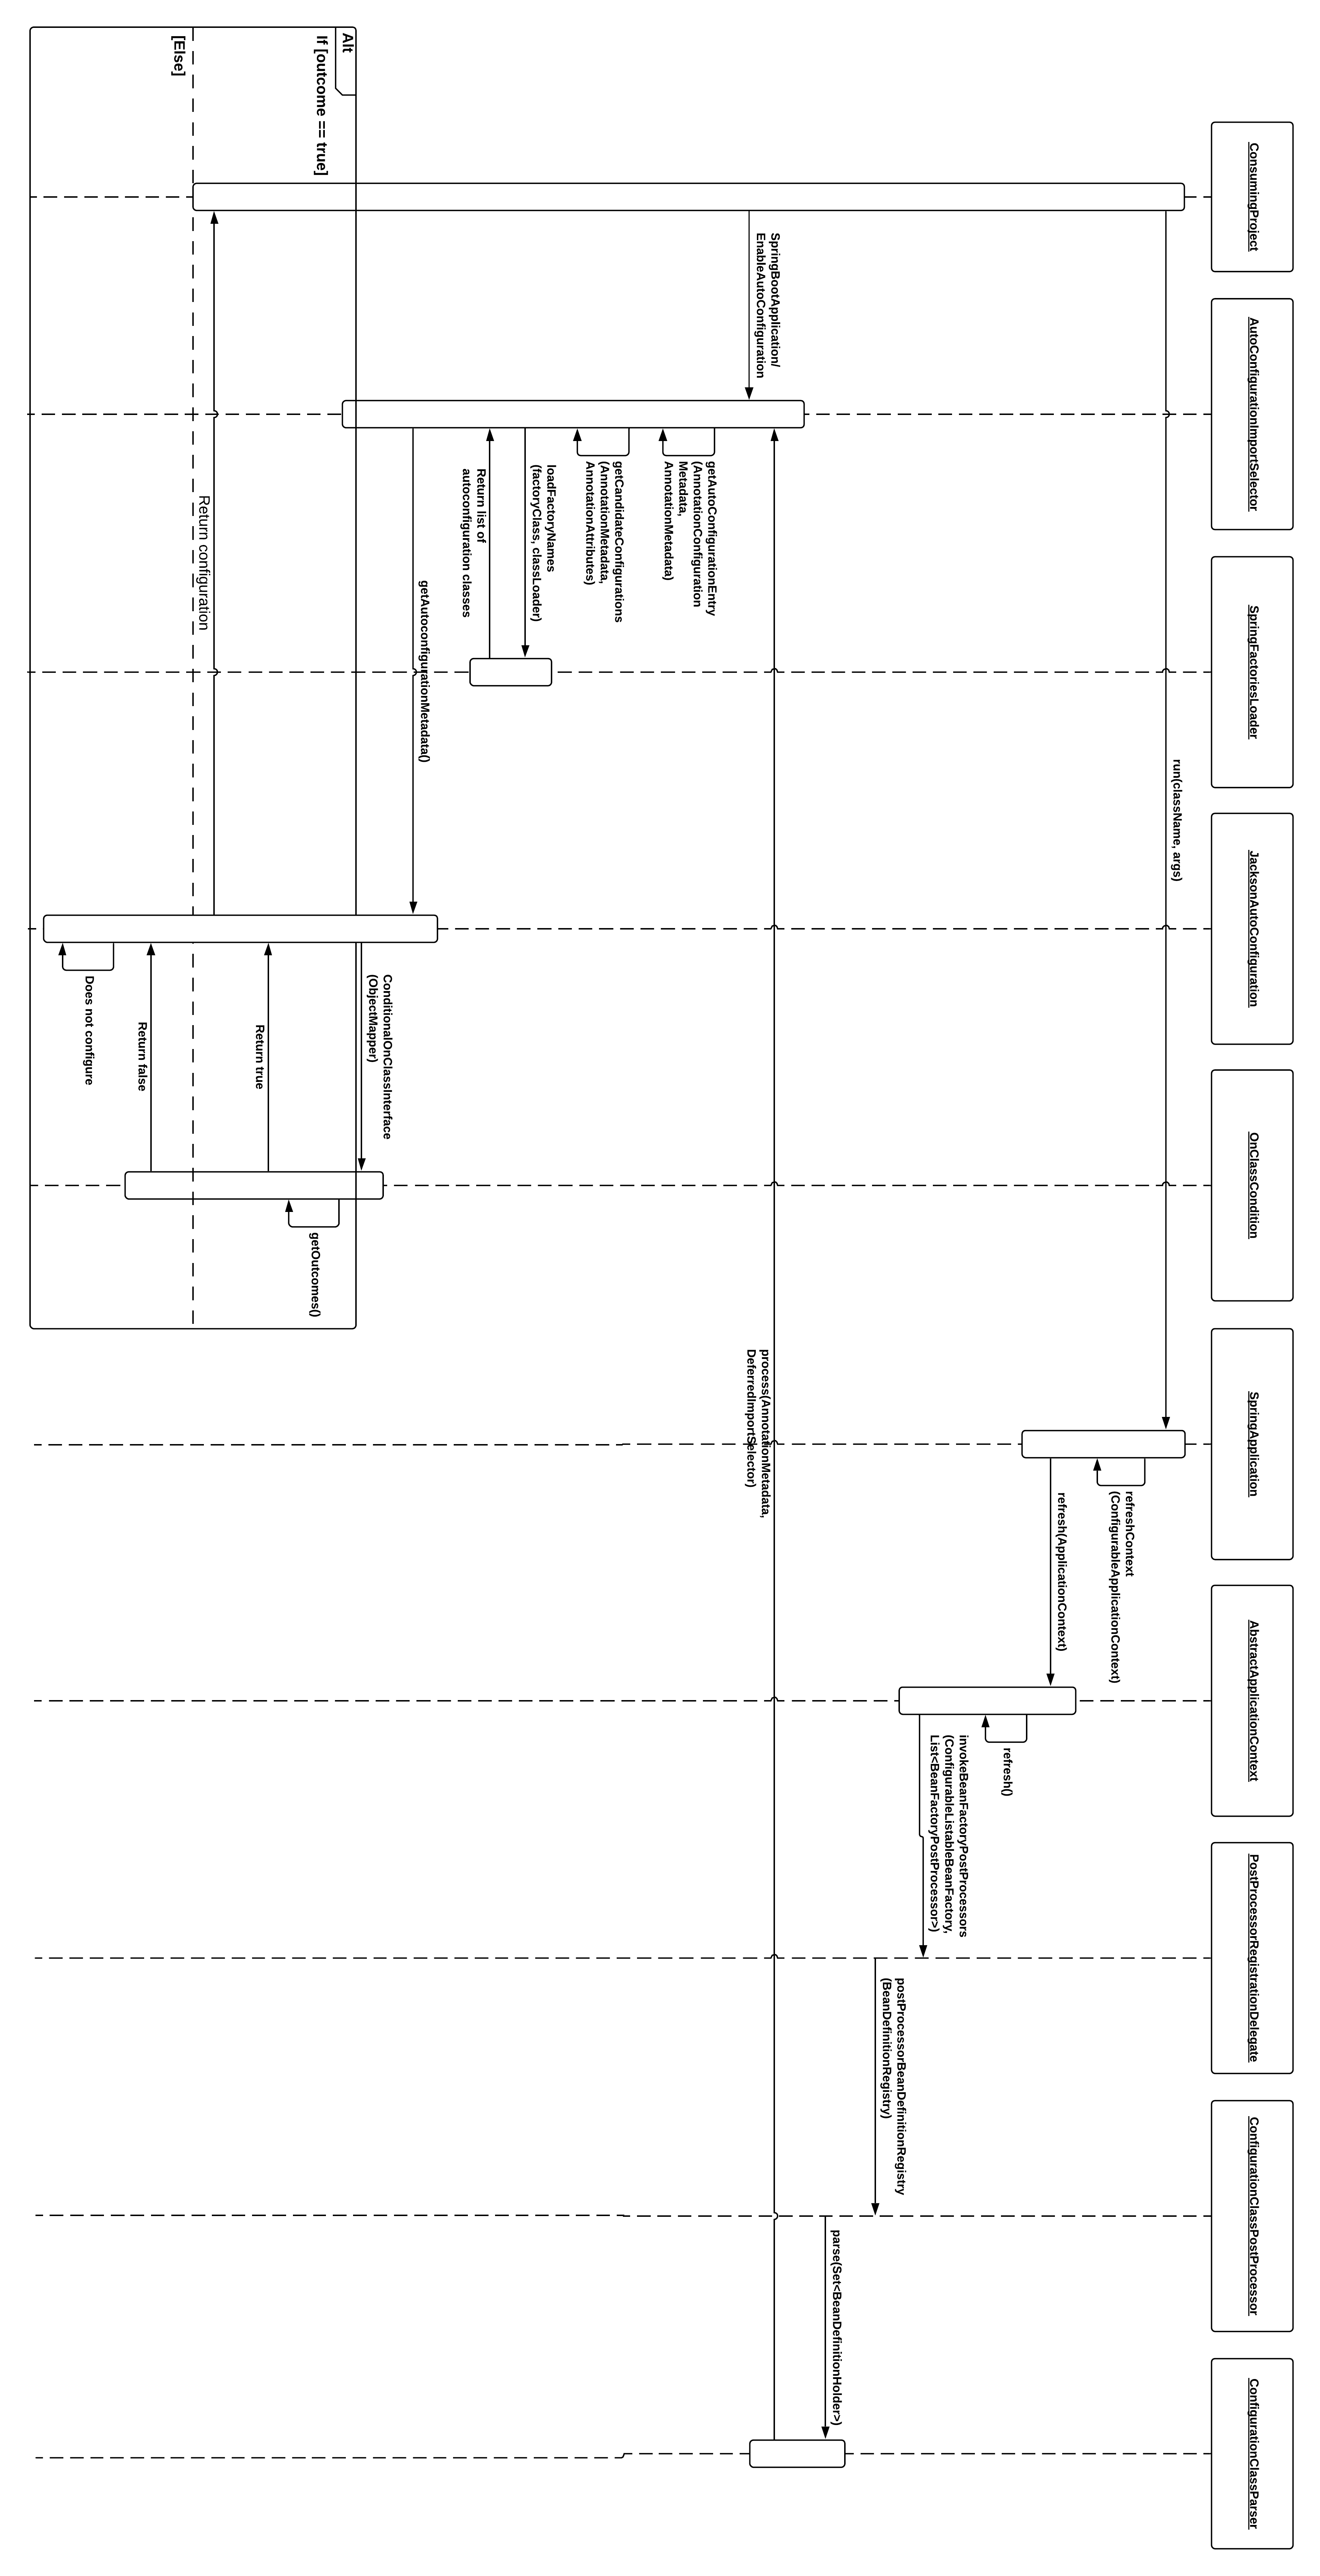
\includegraphics[width=\textwidth, height=.85\textheight, keepaspectratio]{content/architectural-views-top-level/auto-configuration.png}
    \caption{Spring Boot Auto-Configuration Based on Classpath Dependencies}
    \label{sequence-diagram-auto-configuration}
\end{figure}

\textbf{Figure~\ref{sequence-diagram-auto-configuration}}: Consuming projects that use Spring Boot's \texttt{@SpringBootApplication} or \texttt{@EnableAutoConfiguration} will be able to auto-configure their application's dependencies. The figure shows that we are auto-configuring \texttt{Jackson} -- which is a serializer and deserializer library -- in which the \texttt{JacksonAutoConfiguration} class will apply configurations of the \texttt{Jackson} dependency declared in the classpath. The consuming project will use the \texttt{SpringApplication}'s \texttt{run()} method which refreshes the \texttt{ApplicationContext} and eventually invokes the \texttt{AutoConfigurationImportSelector.process()} method. This method will iterate over the pre-defined list of auto-configuration classes defined in the \texttt{spring.factories} file. For each auto-configuration class, the \texttt{AutoConfigurationImportSelector} class will invoke the \texttt{getAutoConfigurationMetadata()} method to call auto-configuration classes to decipher whether or not to configure the consuming project's dependencies. In this particular instance, the called \texttt{JacksonAutoConfiguration} class uses the interface \texttt{@ConditionalOnClass(ObjectMapper.class)} which checks that the \texttt{ObjectMapper} dependency exists in the classpath. If it does, then the \texttt{JacksonAutoConfiguration} class will return the configurations accordingly.

\begin{figure}[H]
    \centering
    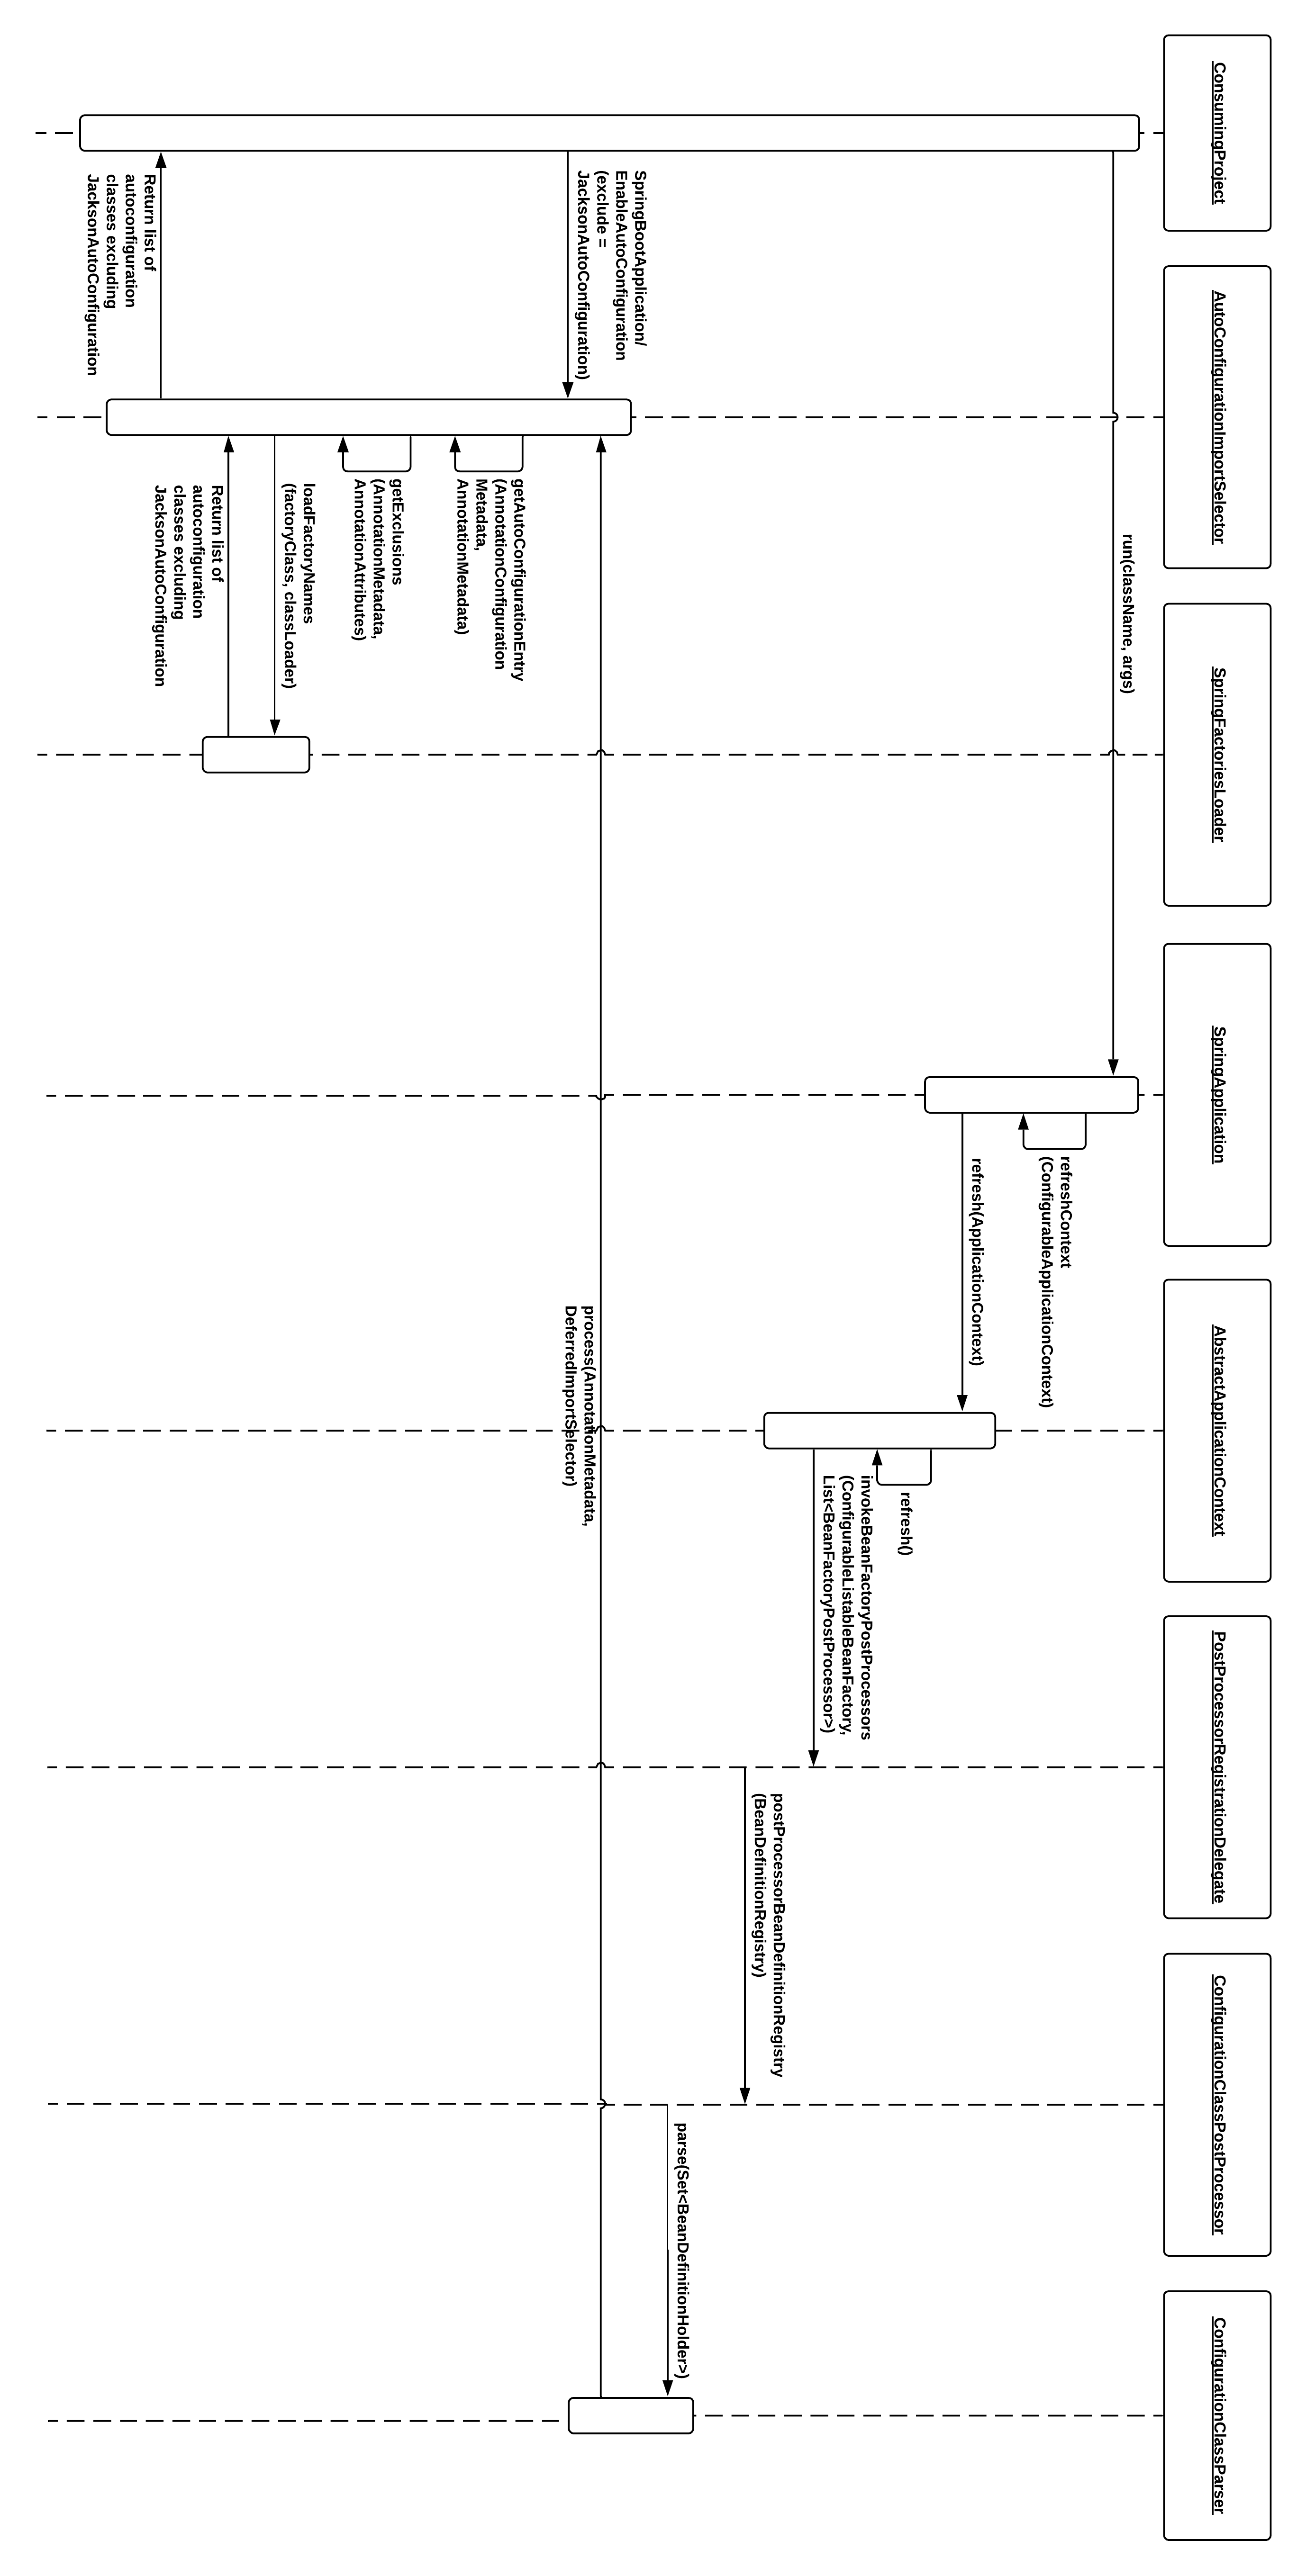
\includegraphics[width=\textwidth, height=\textheight, keepaspectratio]{content/architectural-views-top-level/auto-configuration-exclude.png}
    \caption{Spring Boot Auto-Configuration Exclusion}
    \label{sequence-diagram-auto-configuration-exclude}
\end{figure}

\textbf{Figure~\ref{sequence-diagram-auto-configuration-exclude}}: Consuming projects that use Spring Boot's \texttt{@SpringBootApplication(exclude = JacksonAutoConfiguration.class)} or \texttt{@EnableAutoConfiguration(exclude = JacksonAutoConfiguration.class)} will intently not auto-configure their application's dependency mentioned in the exclude value. The figure shows that we are not auto-configuring \texttt{Jackson}. The consuming project will use the \texttt{SpringApplication}'s \texttt{run()} method which refreshes the \texttt{ApplicationContext} and eventually invokes the \texttt{AutoConfigurationImportSelector.process()} method. This method will iterate over the pre-defined list of auto-configuration classes defined in the \texttt{spring.factories} file excluding the \texttt{JacksonAutoConfiguration} class.

\begin{figure}[H]
    \centering
    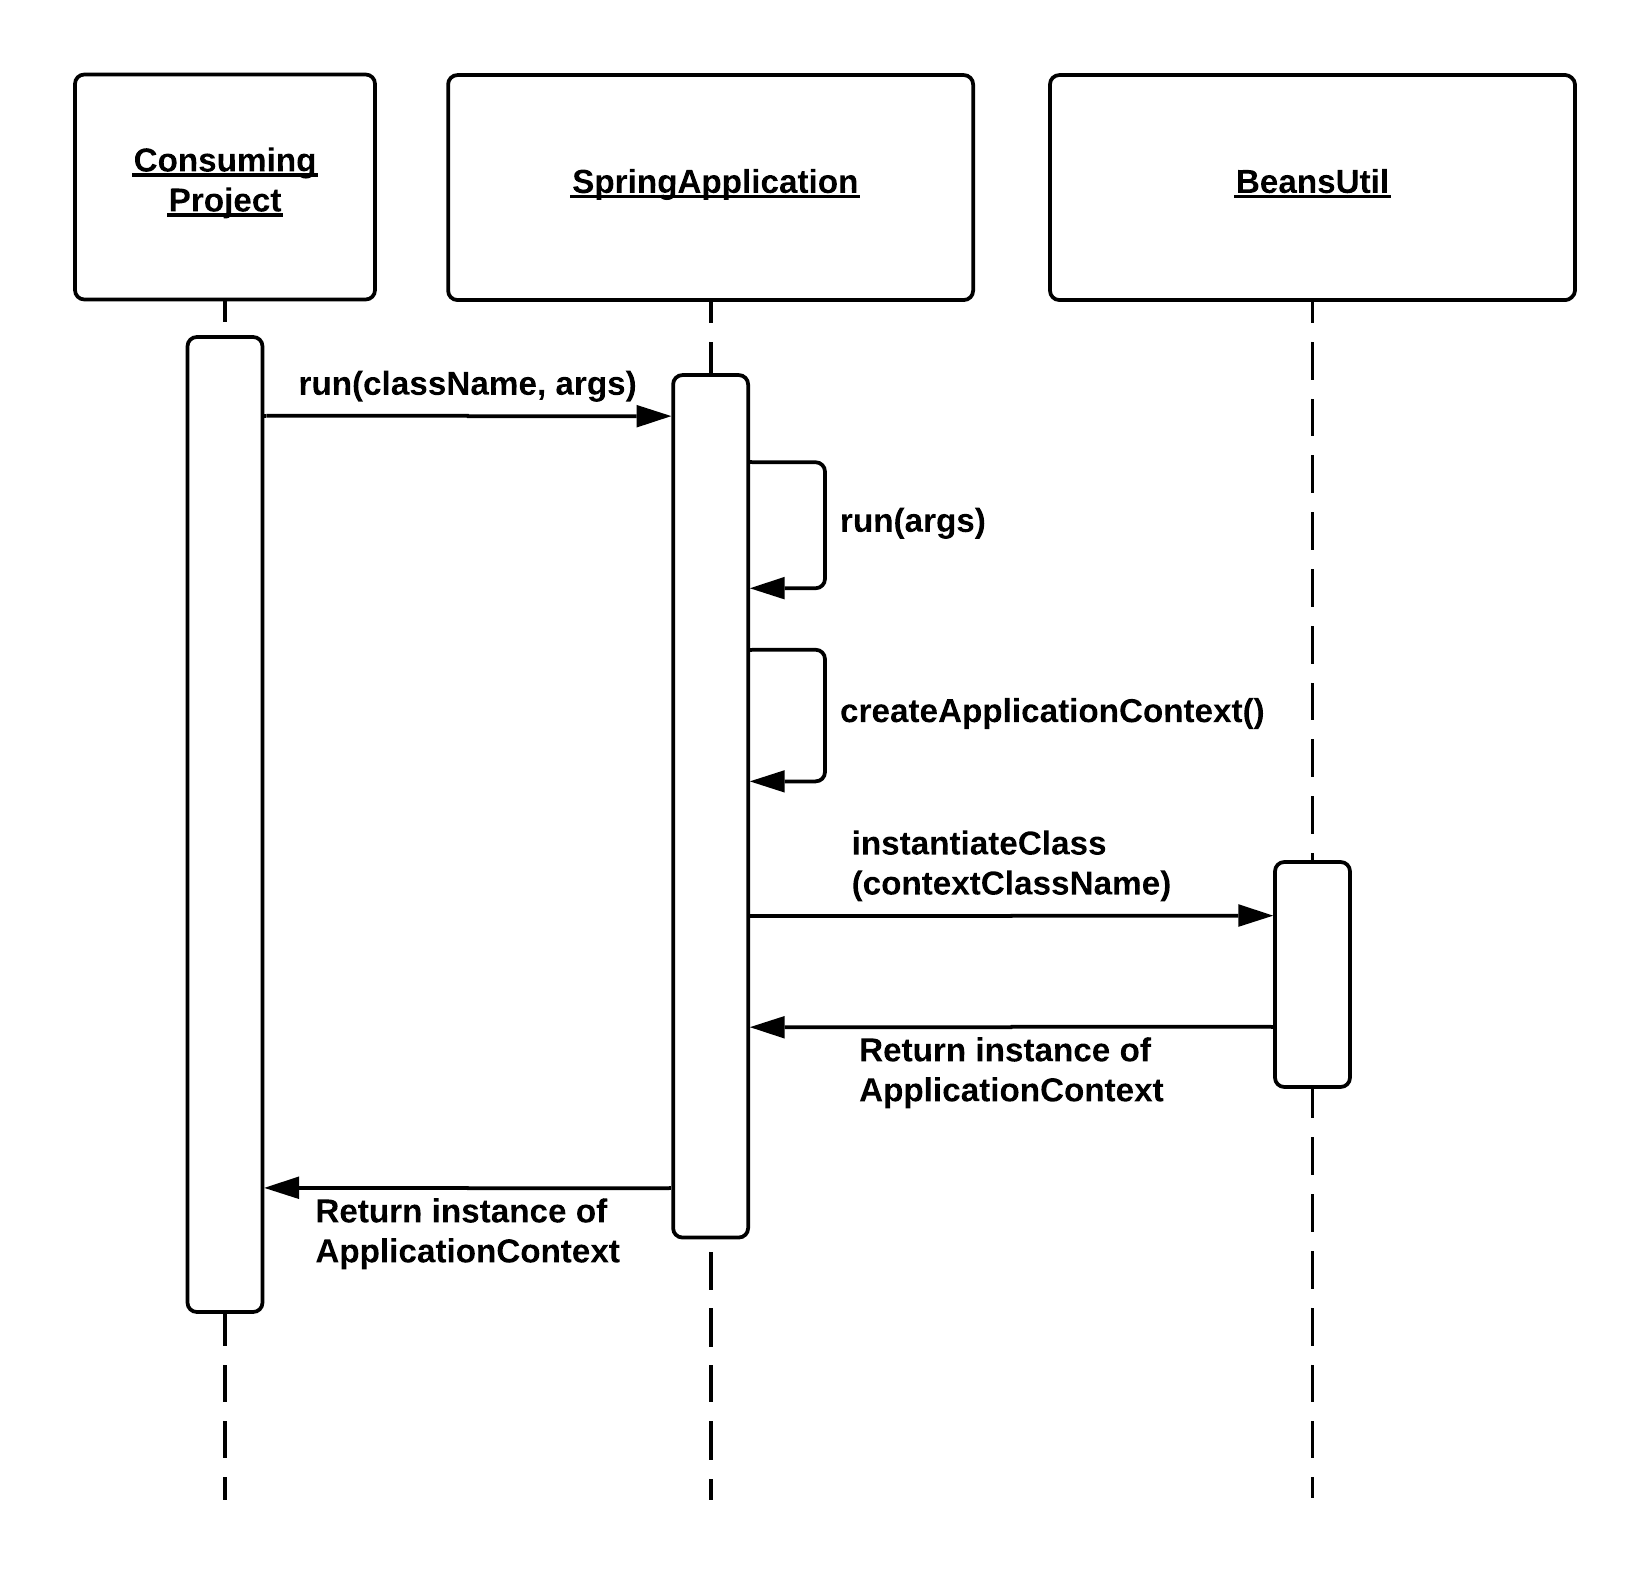
\includegraphics[width=.7\textwidth, height=\textheight, keepaspectratio]{content/architectural-views-top-level/application-context.png}
    \caption{Spring Boot ApplicationContext Creation}
    \label{sequence-diagram-application-context}
\end{figure}

\textbf{Figure~\ref{sequence-diagram-application-context}}: The consuming project will invoke the \texttt{SpringApplication} class' \texttt{run()} method which will self-invoke another overloaded \texttt(run()) method. In this particular \texttt{run()} method, it eventually invokes the \texttt{createApplicationContext()} method that utilizes the strategy pattern to determine the web application type to resolve the context class name. \texttt{SpringApplication} then invokes the \texttt{instantiateClass(contextClassName)} method that returns an \texttt{ApplicationContext} object to the consuming project.

\begin{figure}[H]
    \centering
    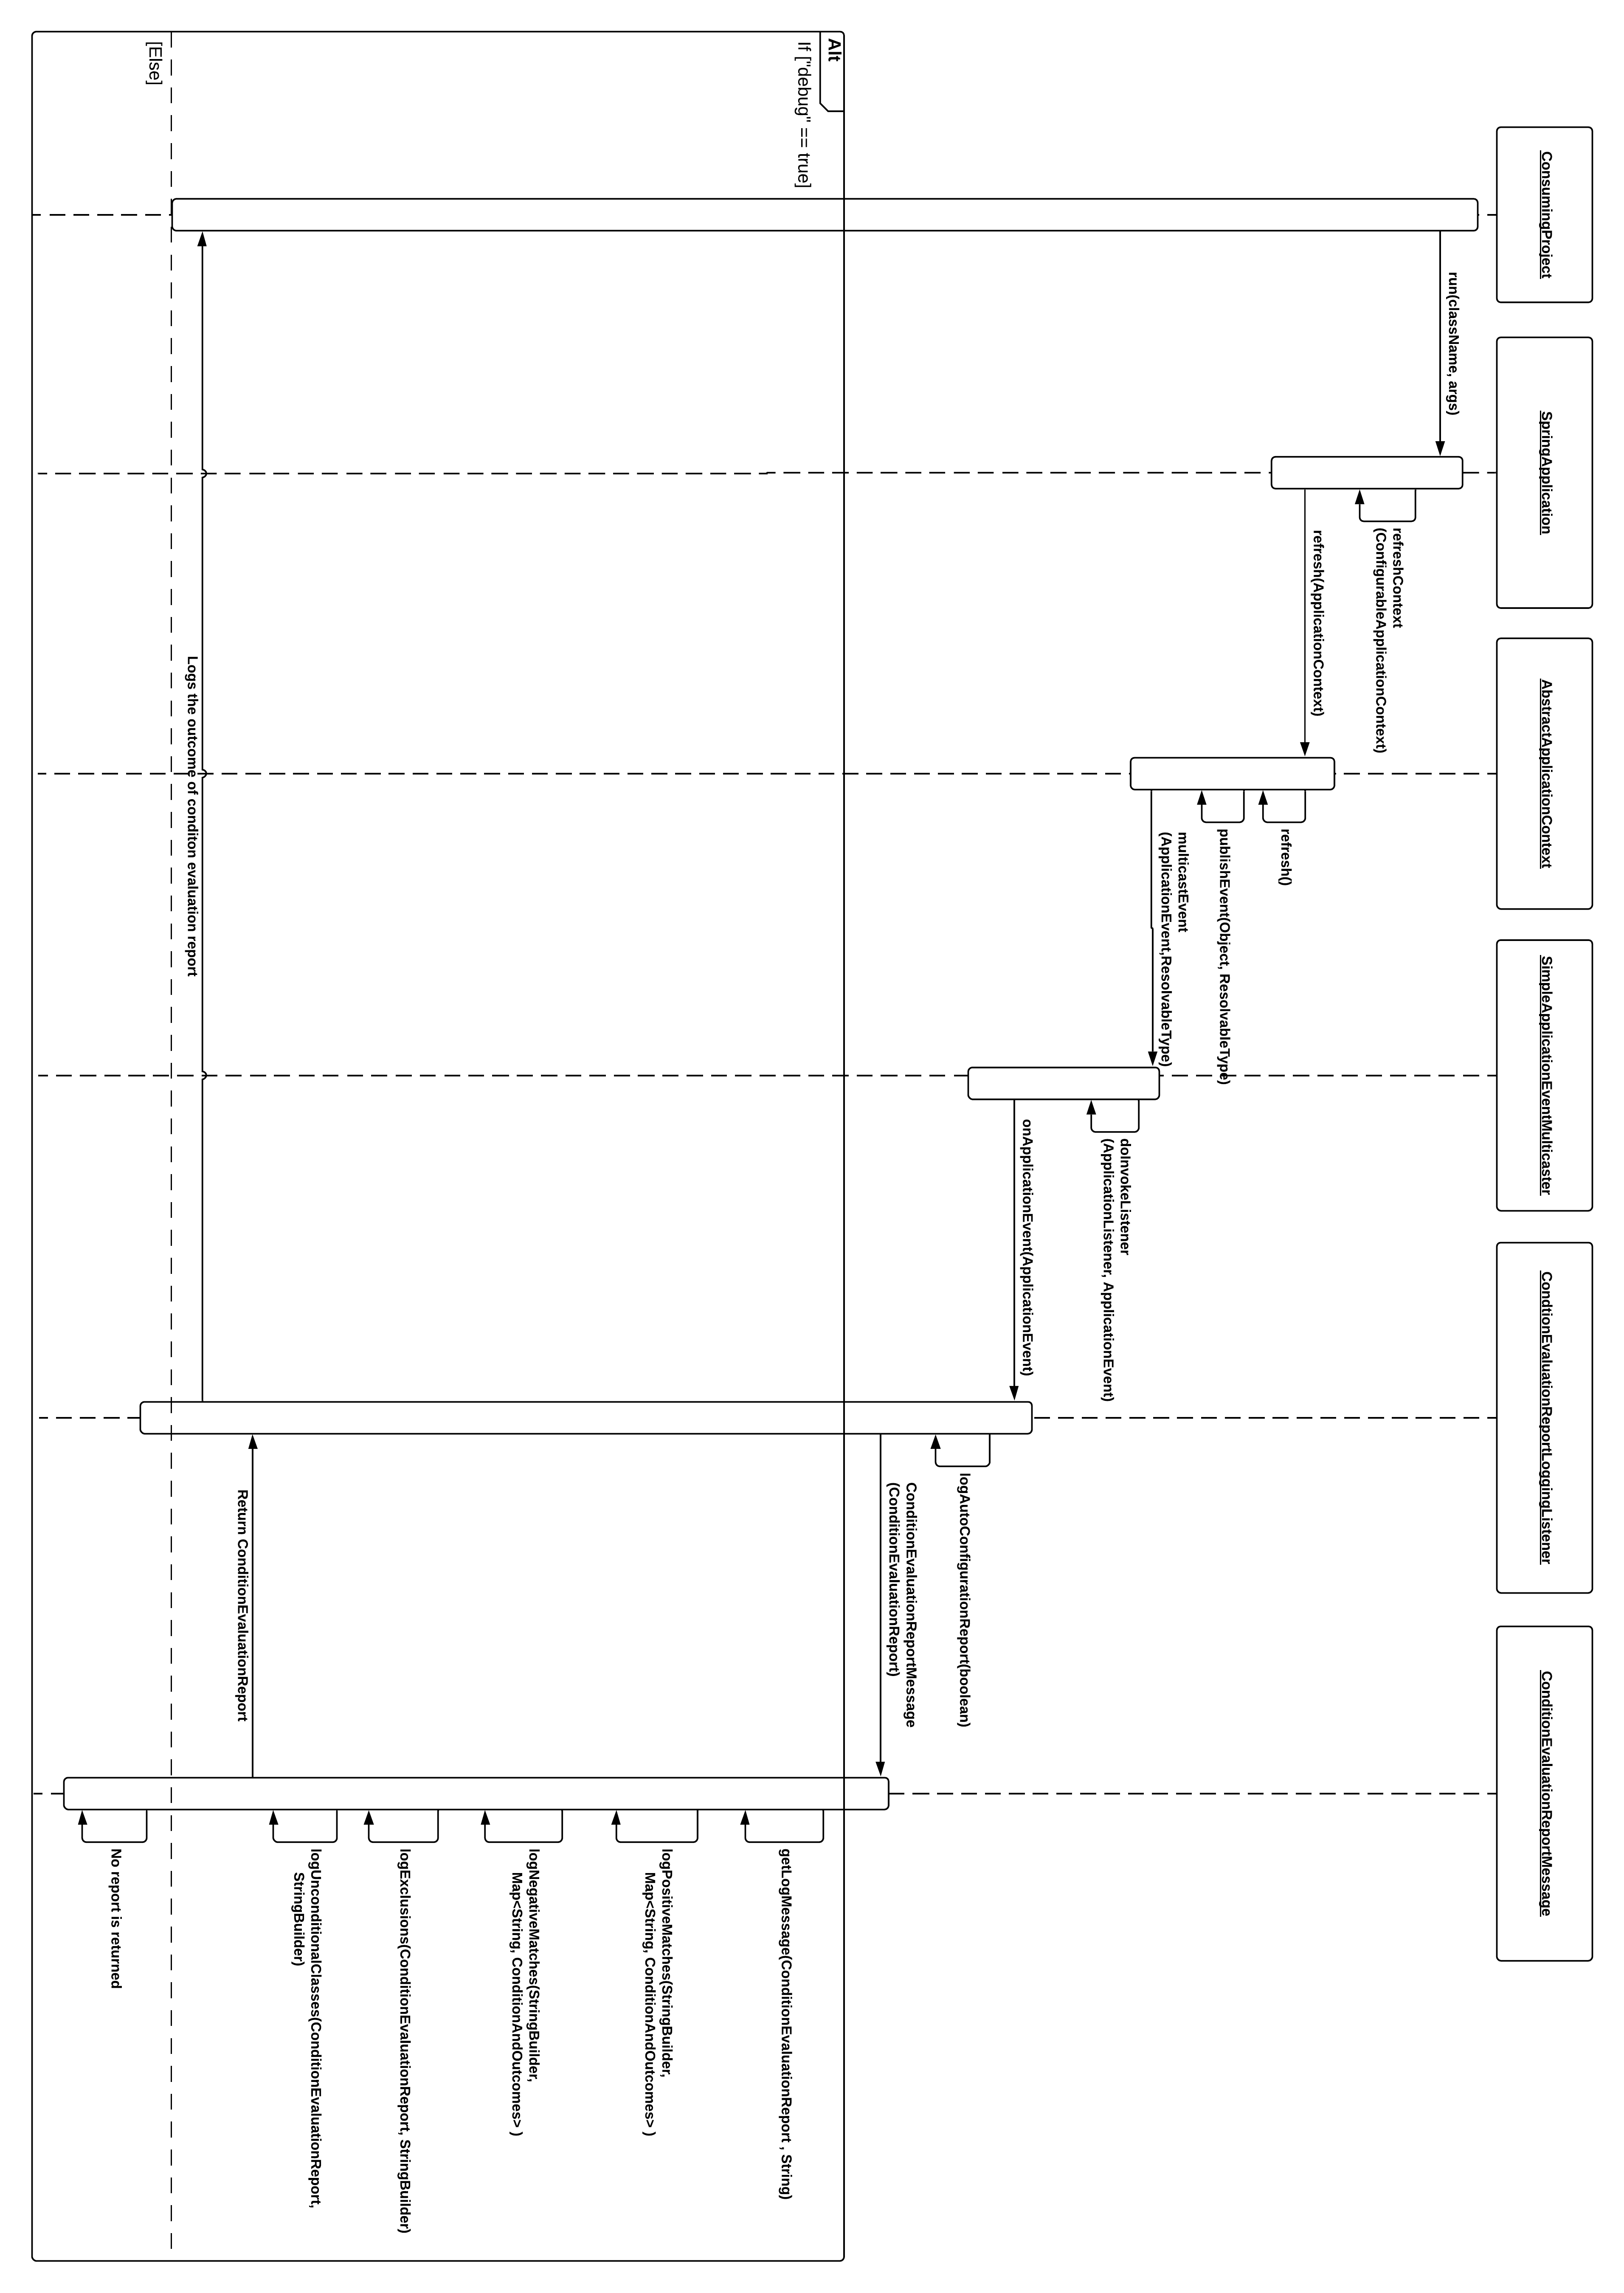
\includegraphics[width=\textwidth, height=\textheight, keepaspectratio]{content/architectural-views-top-level/condition-evaluation-report.png}
    \caption{Spring Boot Condition Evaluation Report}
    \label{sequence-diagram-condition-evaluation-report}
\end{figure}

\textbf{Figure~\ref{sequence-diagram-condition-evaluation-report}}: The consuming project will invoke the \texttt{SpringApplication} class' \texttt{run()} method. Eventually, the \texttt{SimpleApplicationEventMulticaster} class will be invoked by the \texttt{multicastEvent()} method which has an \texttt{ApplicationEvent} argument passed in. The \texttt{SimpleApplicationEventMulticaster} class self-invoke the \texttt{doInvokeListener()} method that listens for the \texttt{ApplicationEvent} which triggers the \texttt{onApplicationEvent()} method, calling all \texttt{*Listener} classes. In this case, the \texttt{ConditionEvaluationReportLoggingListener} class will invoke the \texttt{ConditionEvaluationReportMessage} constructor with the \texttt{ConditionEvaluationReport} as the argument. The \texttt{ConditionEvaluationReportMessage} class will then find the matching outcomes for auto-configuration classes and pre-defined beans when configuring conditional beans. The end result of this process will return the log output of \texttt{ConditionEvaluationReport} if debug is set to true. Otherwise, it will not return the log.

\begin{figure}[H]
    \centering
    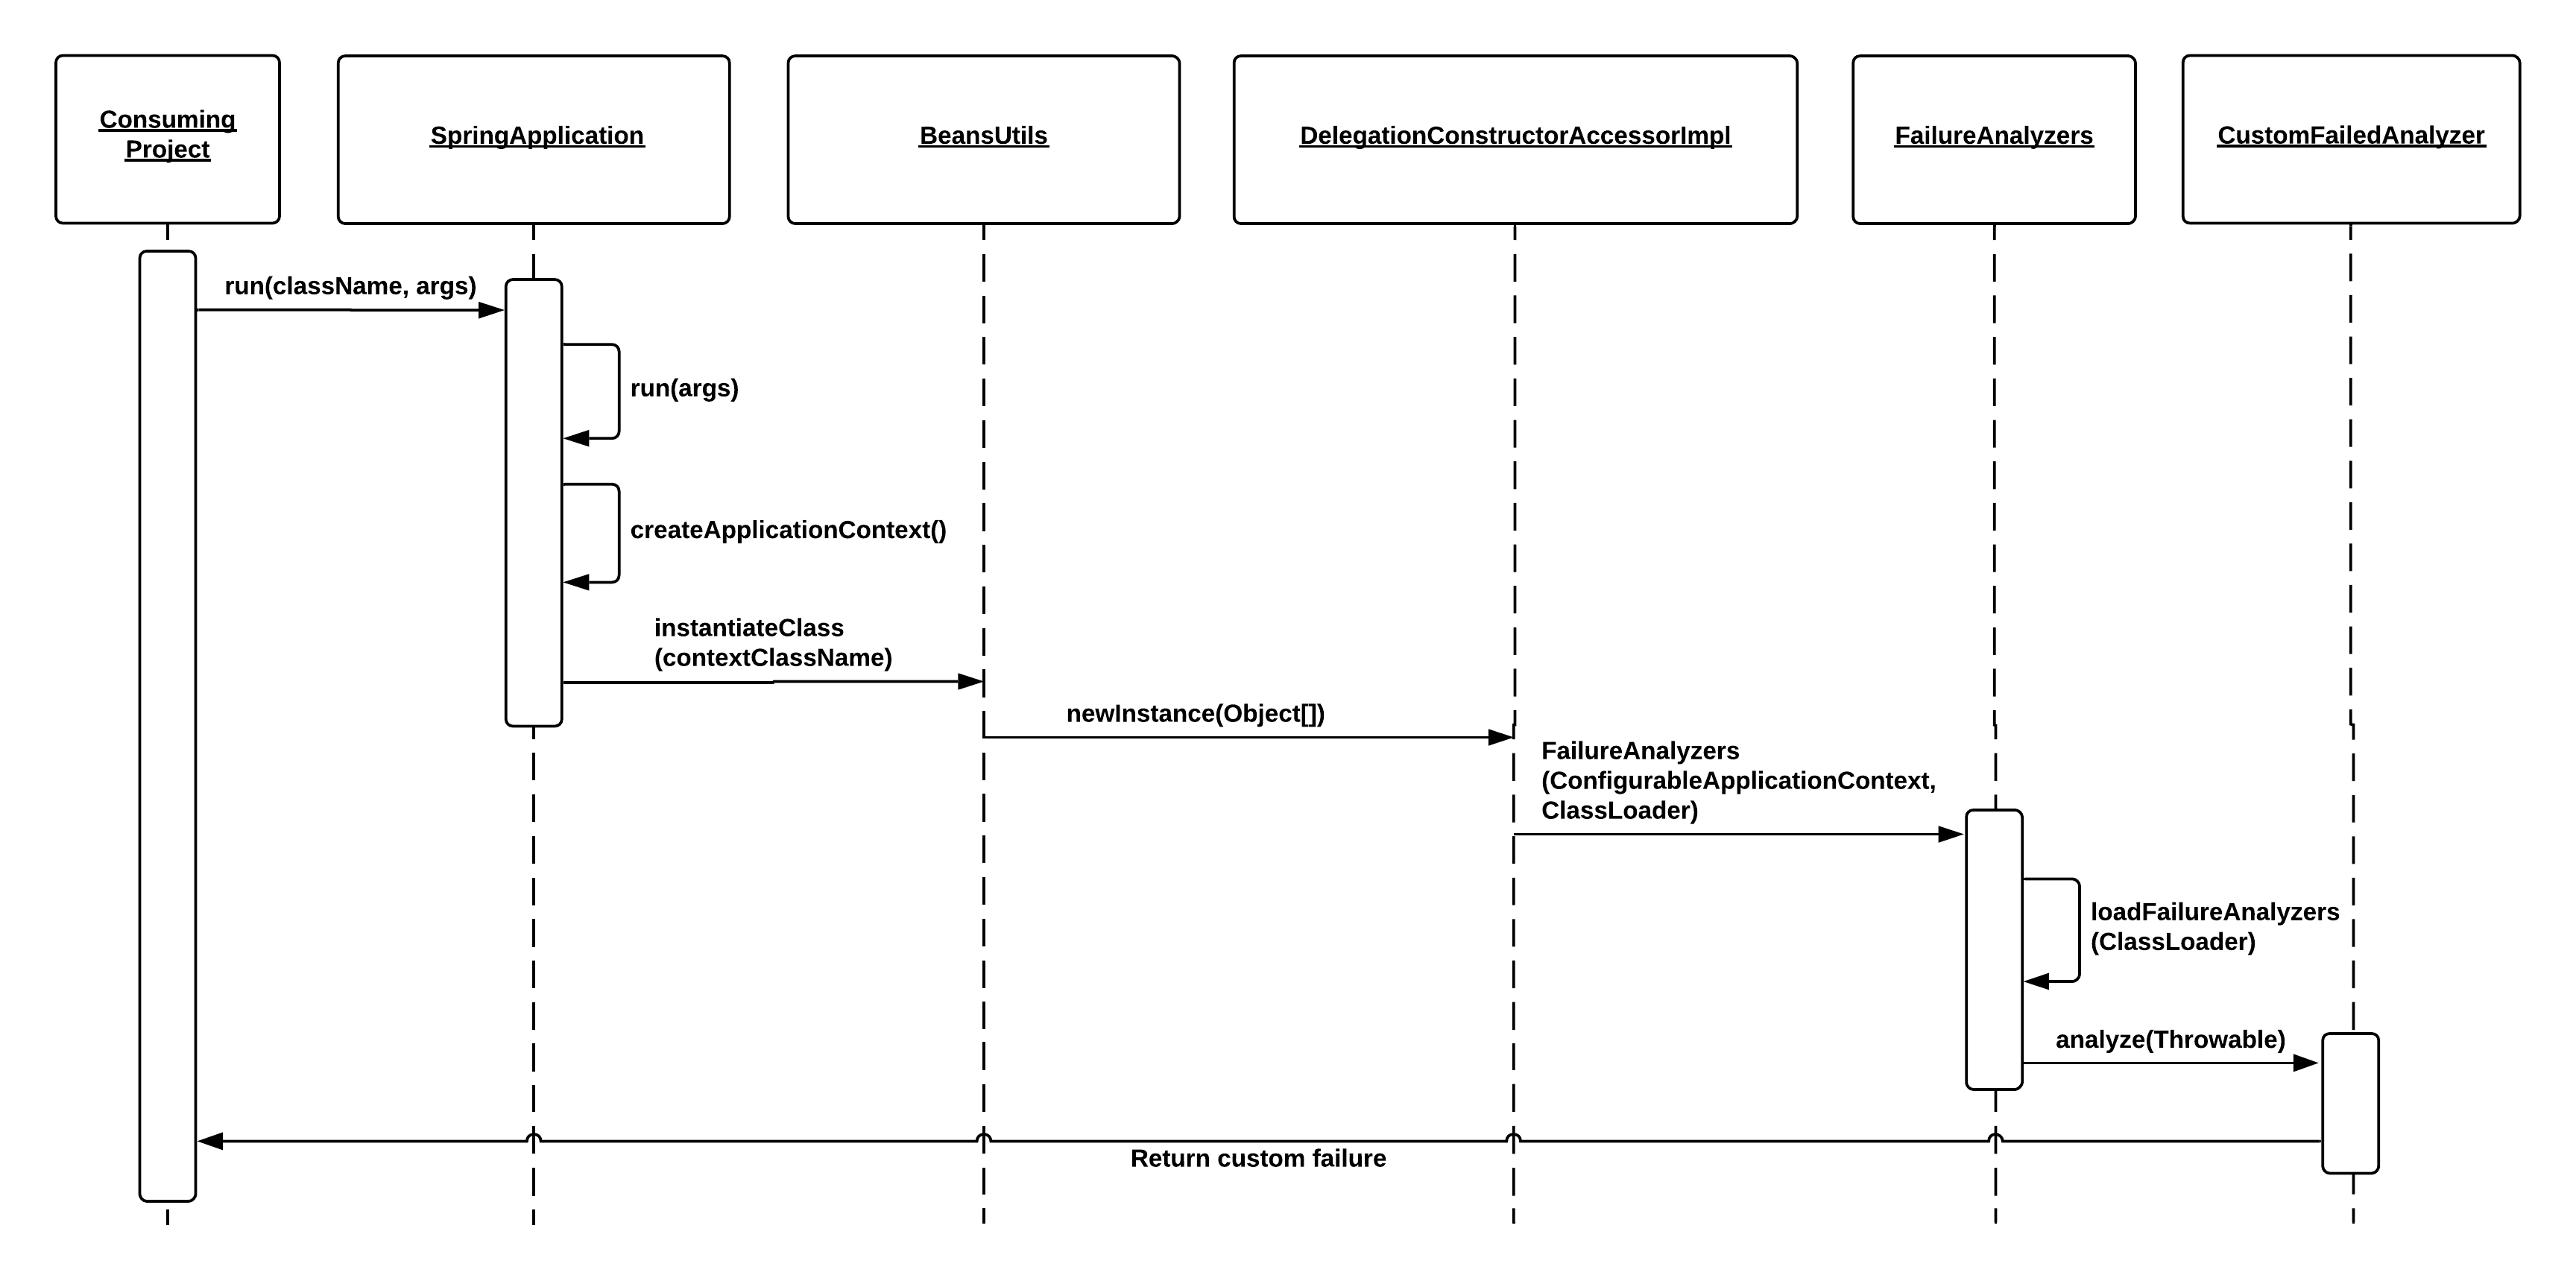
\includegraphics[width=\textwidth, height=\textheight, keepaspectratio]{content/architectural-views-top-level/custom-failure-analyzer.png}
    \caption{Spring Boot Custom Failure Analyzer}
    \label{sequence-diagram-custom-failure-analyzer}
\end{figure}

\textbf{Figure~\ref{sequence-diagram-custom-failure-analyzer}}: The consuming project will invoke the \texttt{SpringApplication} class' \texttt{run()} method and eventually the \texttt{instantiateClass()} method of the \texttt{BeanUtils} class will be invoked. The \texttt{BeanUtils} class will invoke the \texttt{newInstance()} method of the \texttt{DelegationConstructorAccessorImpl} class. This class will invoke the constructor of \texttt{FailureAnalyzers} in which the \texttt{FailureAnalyzers} class will iterate through the list of failure analyzer classes defined in the \texttt{spring.factories} file. In this figure, \texttt{CustomFailedAnalyzer} is a user-defined class which overrides the \texttt{analyze()} method of \texttt{FailureAnalyzers} class. The overridden method of \texttt{analyze()} will return the custom failure as defined in the \texttt{CustomFailedAnalyzer} class.
